\documentclass[9pt,a4paper,twoside]{tau}
\usepackage[english]{babel}
\usepackage{tauenvs}

%----------------------------------------------------------
% TITLE
%----------------------------------------------------------

\title{Investigative Report of Franklin Resources Inc. [stock:BEN]from April 2022 to April 2024}

%----------------------------------------------------------
% AUTHORS, AFFILIATIONS AND PROFESSOR
%----------------------------------------------------------

\author[a,1]{Bucsa, Justin}

%----------------------------------------------------------

\affil[a]{Stealth}
\professor{}

%----------------------------------------------------------
% FOOTER INFORMATION
%----------------------------------------------------------

\institution{Stealth}
\ftitle{}
\date{April 19, 2024}
\etal{Bucsa}
\course{}

%----------------------------------------------------------
% ABSTRACT
%----------------------------------------------------------

\begin{abstract}    
    This report provides a comprehensive analysis of Franklin Resources Inc. (BEN) as a potential investment opportunity. It examines the company's performance over a two-year period (April 2022 - April 2024), encompassing historical background, strategic goals, and major shareholder structure. We will delve into market data to understand BEN's price movements and analyze key events that transpired within the past year (April 2023 - April 2024) to assess their impact. Finally, the report culminates in a holistic evaluation of Franklin Resources Inc.'s investment potential.
\end{abstract}

%----------------------------------------------------------
% \keywords{}
%----------------------------------------------------------

\begin{document}
		
	\maketitle
	\thispagestyle{firststyle}
	\tauabstract
	\tableofcontents

%----------------------------------------------------------

\section{Introduction}

    \taustart{F}ranklin Resources Inc. [NYSE:BEN], is one of the world's largest investment managers, is better known as Franklin Templeton. It currectly over sees \$1.6 trillion in total assets under management, over 1400 investment professionals in 25 counties and over 9000 employees globally. In this report will first discuss

\section{History}
    Franklin Resources boasts a rich history dating back to 1947, when it began operations in the investment management field. The company initially focused on mutual funds, offering both fixed income and equity options (growth and value-oriented). Through strategic acquisitions, Franklin has continuously expanded its reach and expertise. Notable additions include:

    - 1992: Templeton, a global investment firm, bringing international investment capabilities.
    
    - 1996: Franklin Mutual Series, further solidifying its mutual fund portfolio.

    - 2000 \& 2001: Acquisitions like Franklin Bissett Canadian and Fiduciary Trust International broadened their offerings to include Canadian investment management and trust services.
    
    - 2019-2022: A period of significant expansion, with acquisitions like Benefit Street Partners (alternative credit), Athena Capital Advisors (wealth management), Legg Mason (global investments), O’Shaughnessy Asset Management (quantitative assets), Lexington Partners (alternative investments), and Alcentra (alternative credit).
    
    This strategic growth through acquisitions has transformed Franklin Resources into a leading global investment management firm with a diverse range of offerings to meet evolving investor needs.
    
\section{Events}

    \subsection{May 2023 - Acquisition of Putnam Investments Announced}
	
        Franklin Resources Inc. announced a significant acquisition in May 2023, entering into a definitive agreement to acquire Putnam Investments from Great-West Lifeco. Inc. (Great-West), a member of the prominent Power Corporation group. This strategic move strengthens Franklin Templeton's position in the asset management industry. Great-West and Power Corporation are leaders in global insurance, retirement, wealth management, and asset management, aligning well with Franklin Templeton's existing strengths. The acquisition was expected to close in the first quarter of fiscal year 2024, subject to customary closing conditions.

    \subsection{January 2024 - Acquisition of Putnam Investments Completed}
	
        Franklin Resources Inc. successfully completed the acquisition of Putnam Investments, expanding its global footprint and AUM (Assets Under Management). This strategic move solidified Franklin Resources' position as a leading investment management firm.
    
    \subsection{Insider Sales}
    Below is a list of Insider stock sales from members of Franklin Resources Inc. exectives and board of directors from 2022-04-20 to 2024-04-20.
    
    
    \begin{figure}[H]
        \centering
        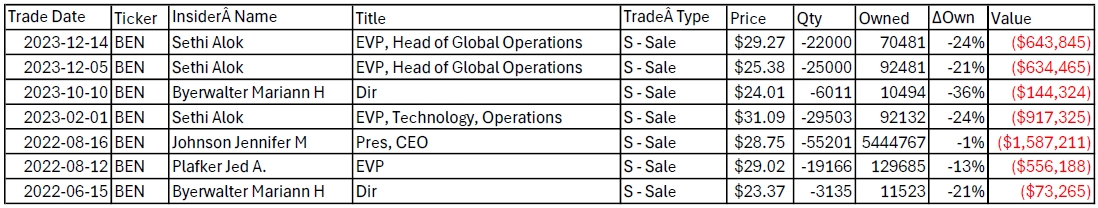
\includegraphics[width=0.95\columnwidth]{images/InsiderTrades.jpg}
        \caption{This is a table of Insider Trades from 2022-04-20 to 2024-04-20.}
        \label{fig:figure}
    \end{figure}

\section{Ownership Distribution}
    \subsection{Breakdown}
    Franklin Resources Inc. [NYSE:BEN] is divided into four categories of ownership: Insiders, Mutual Funds, Other Institional Investors, and Public Companies and Individual Investors. The pie chart below shows the distribution of ownership, were Insiders own the most at 40.88\% followed by Public Companies and Individual Investors at 25.85\%, Other Institional Investors at 19.77\% and finally Mutual Funds at 13.50\%.

    \begin{figure}[H]
        \centering
        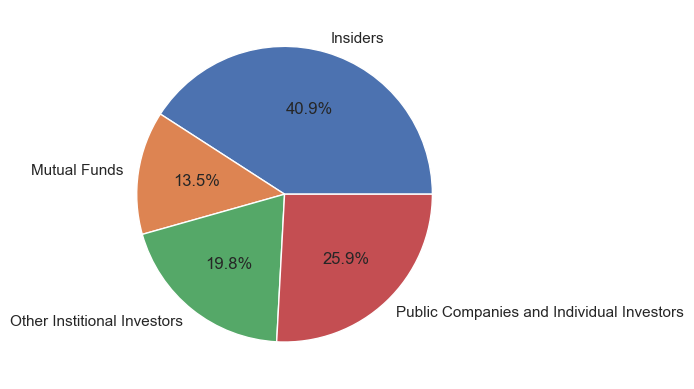
\includegraphics[width=0.85\columnwidth]{images/OwnershipPieChart.png}
        \caption{This chart represents how the shares of BEN are divided up as of 2024-04-20.}
        \label{fig:figure}
    \end{figure}

    \subsection{Concerns}
    
    You're right, Franklin Resources Inc. (NYSE: BEN) could be susceptible to immediate stock price swings. With a large portion of the ownership concentrated in insiders, public companies, and other institutional investors (holdings totaling 86.5\%) compared to mutual funds, the stock price could react more dramatically if these major investors decide to sell.  This concentration of ownership suggests that BEN might be a more stable choice for short-term investment strategies, but for long-term investors, the vulnerability to large investor sentiment should be a consideration

\section{Market Analysis}
    \subsection{Introduction to Market Analysis}
    This section will be focused on examining the Closing Price and Quarterly Revenue of Franklin Resources Inc. (NYSE: BEN) from 2022-04-20 to 2024-04-20. We will discuss possible impacts to each respectively and then compare both together. 
    
    \subsection{Closing Price}
    Below is the Closing Cost of Franklin Resources Inc. (NYSE: BEN) per month from 2022-04-20 to 2024-04-20.
        \begin{figure}[H]
            \centering
            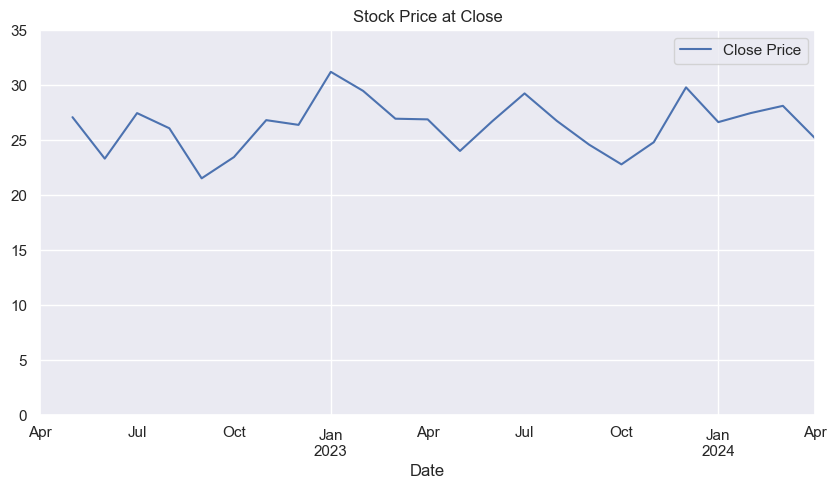
\includegraphics[width=0.85\columnwidth]{images/CloseDataSet1mo.png}
            \caption{This chart represents the Closing Stock Price per Month from 2022-04-20 to 2024-04-20.}
            \label{fig:figure}
        \end{figure}
    The price appears to be in a flux of plus or minus \$5.00 every quarter. In fact, if we look at the daily trades, we can see the jumps more clearly occur at a quartly period. 
        \begin{figure}[H]
            \centering
            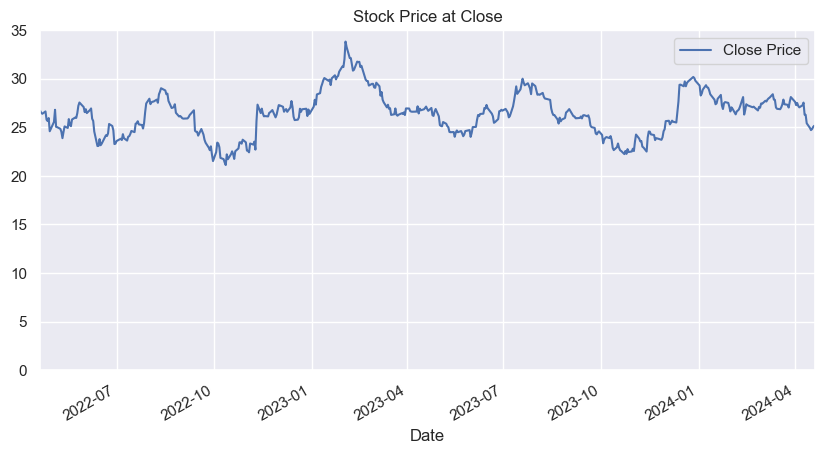
\includegraphics[width=0.85\columnwidth]{images/CloseDataSet1d.png}
            \caption{This chart represents the Closing Stock Price per Day from 2022-04-20 to 2024-04-20.}
            \label{fig:figure}
        \end{figure}
    If we compare the two charts together, we can see the month average trails the daily report due to this large jumps in the Closing Price.
        \begin{figure}[H]
            \centering
            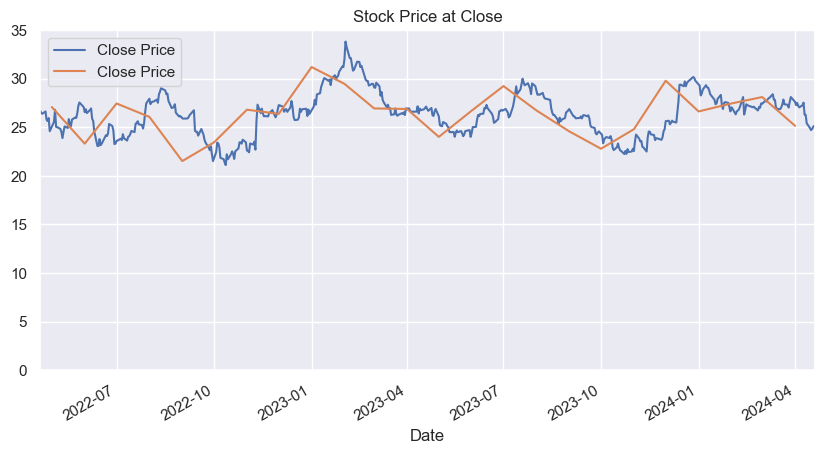
\includegraphics[width=0.85\columnwidth]{images/CloseDataSet1dvs1mo.png}
            \caption{This chart represents the Closing Stock Price per Day vs. Closing Stock Price per Month from 2022-04-20 to 2024-04-20.}
            \label{fig:figure}
        \end{figure}
    This leads us to comclude there is a market force acting on the start that makes it visiable for a daily trading over monthly trading. 

    Let us continue into the Quarterly Revenue reports.

    \subsubsection{Quarterly Revenue}
        Since Franklin Resources Inc. [NYSE:BEN] does have over \$1.6 trillion in asset under managerment, we can see their earnings report show a profit of sometimes breaking \$200 billion in recently quarter. Below is a chart show the recent Quarter Revenue from 2022-04-20 to 2024-04-20.
            \begin{figure}[H]
                \centering
                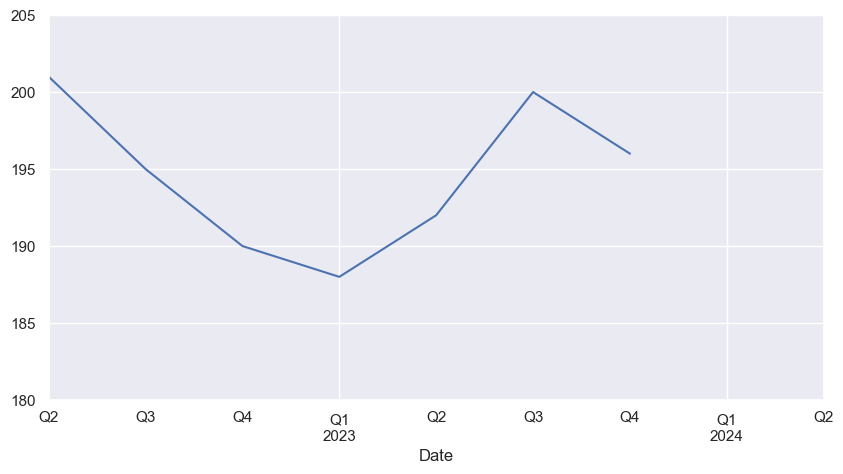
\includegraphics[width=0.85\columnwidth]{images/EarningByQt.png}
                \caption{This chart represents the report earning in Billions over the quarters from 2022-04-20 to 2024-04-20.}
                \label{fig:figure}
            \end{figure}
        It appears that the revenue of Franklin Resources Inc. [NYSE:BEN] does fluxate plus or minus \$5 billion, that's smaller rate of change than the stocks fluxates.  
            
        
        
        \begin{figure}[H]
                \centering
                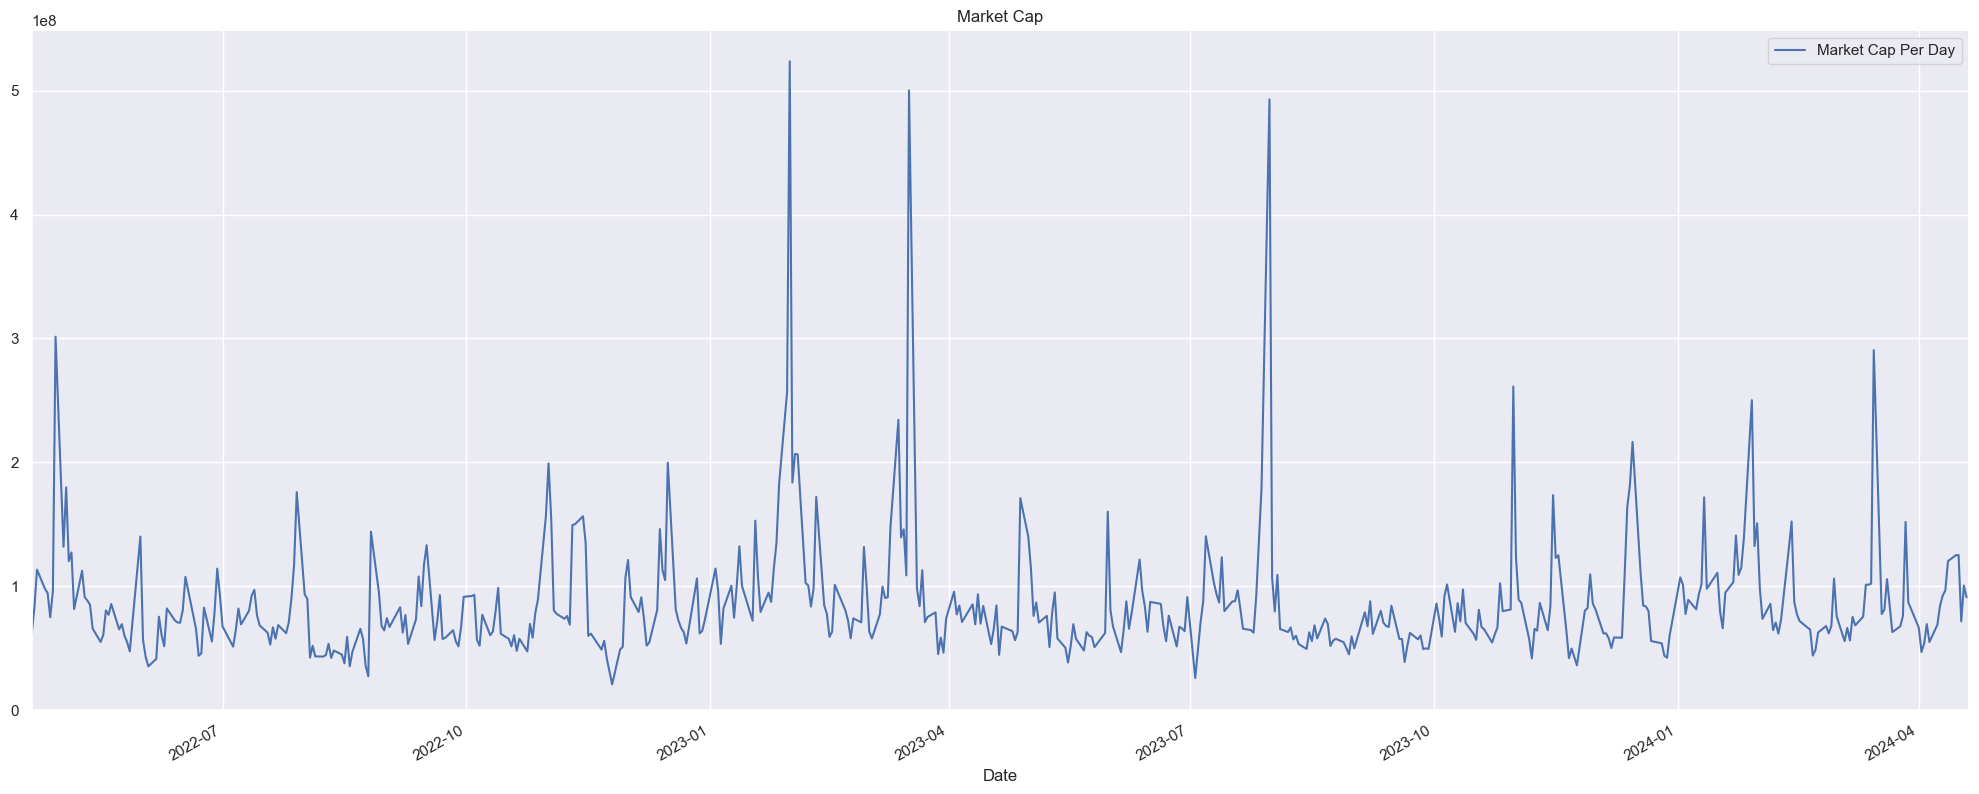
\includegraphics[width=0.85\columnwidth]{images/MarketCap1d.png}
                \caption{This chart represents the Martet Cap. per Day from 2022-04-20 to 2024-04-20.}
                \label{fig:figure}
            \end{figure}


            \begin{figure}[H]
                \centering
                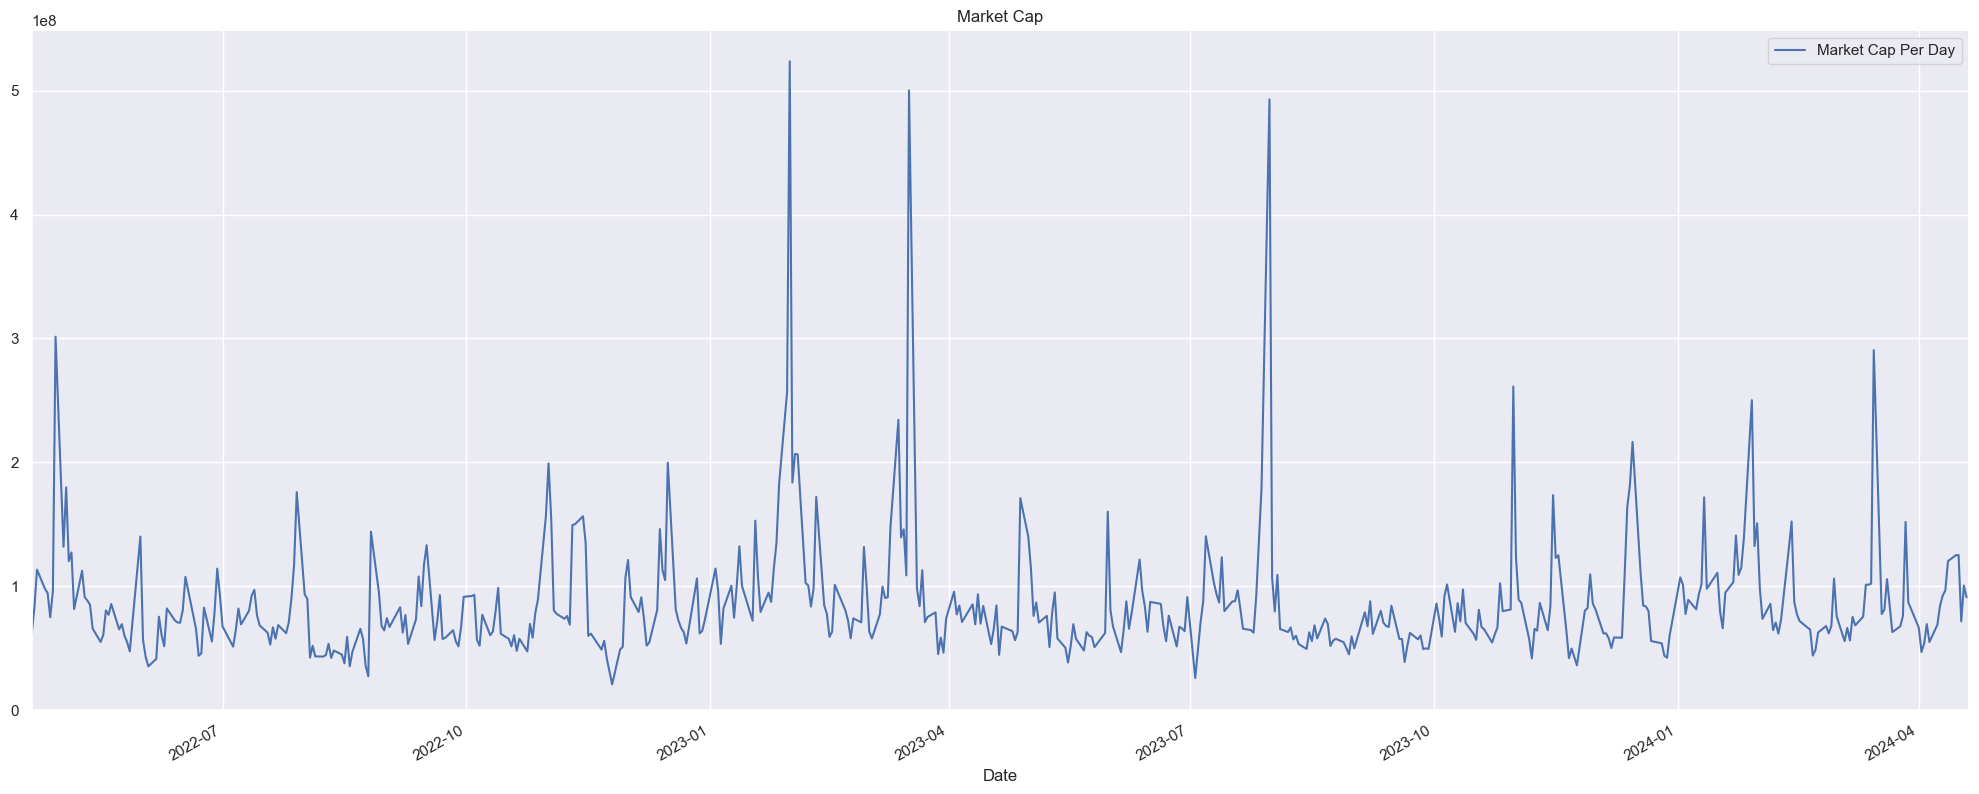
\includegraphics[width=0.85\columnwidth]{images/MarketCap1d.png}
                \caption{This chart represents the Martet Cap. per Month from 2022-04-20 to 2024-04-20.}
                \label{fig:figure}
            \end{figure}


            \begin{figure}[H]
                \centering
                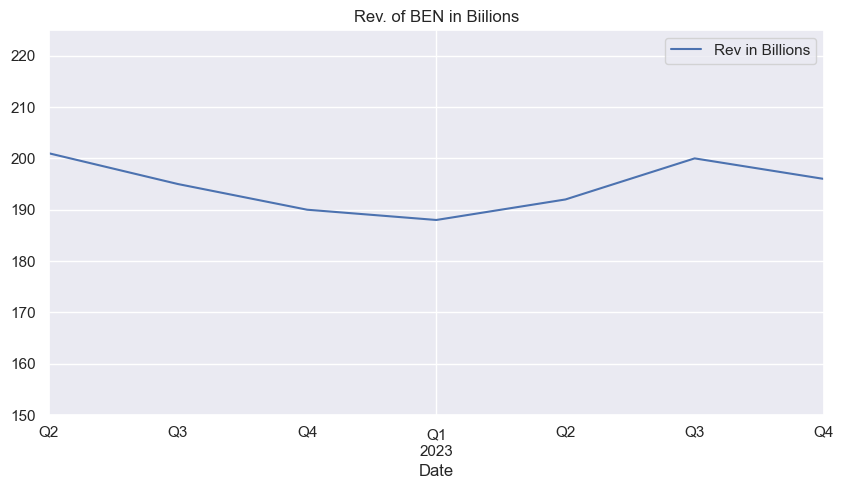
\includegraphics[width=0.85\columnwidth]{images/RevInBillions.png}
                \caption{This chart represents the report Revenue in Billions per quarter from 2022-04-20 to 2024-04-20.}
                \label{fig:figure}
            \end{figure}

            \begin{figure}[H]
                \centering
                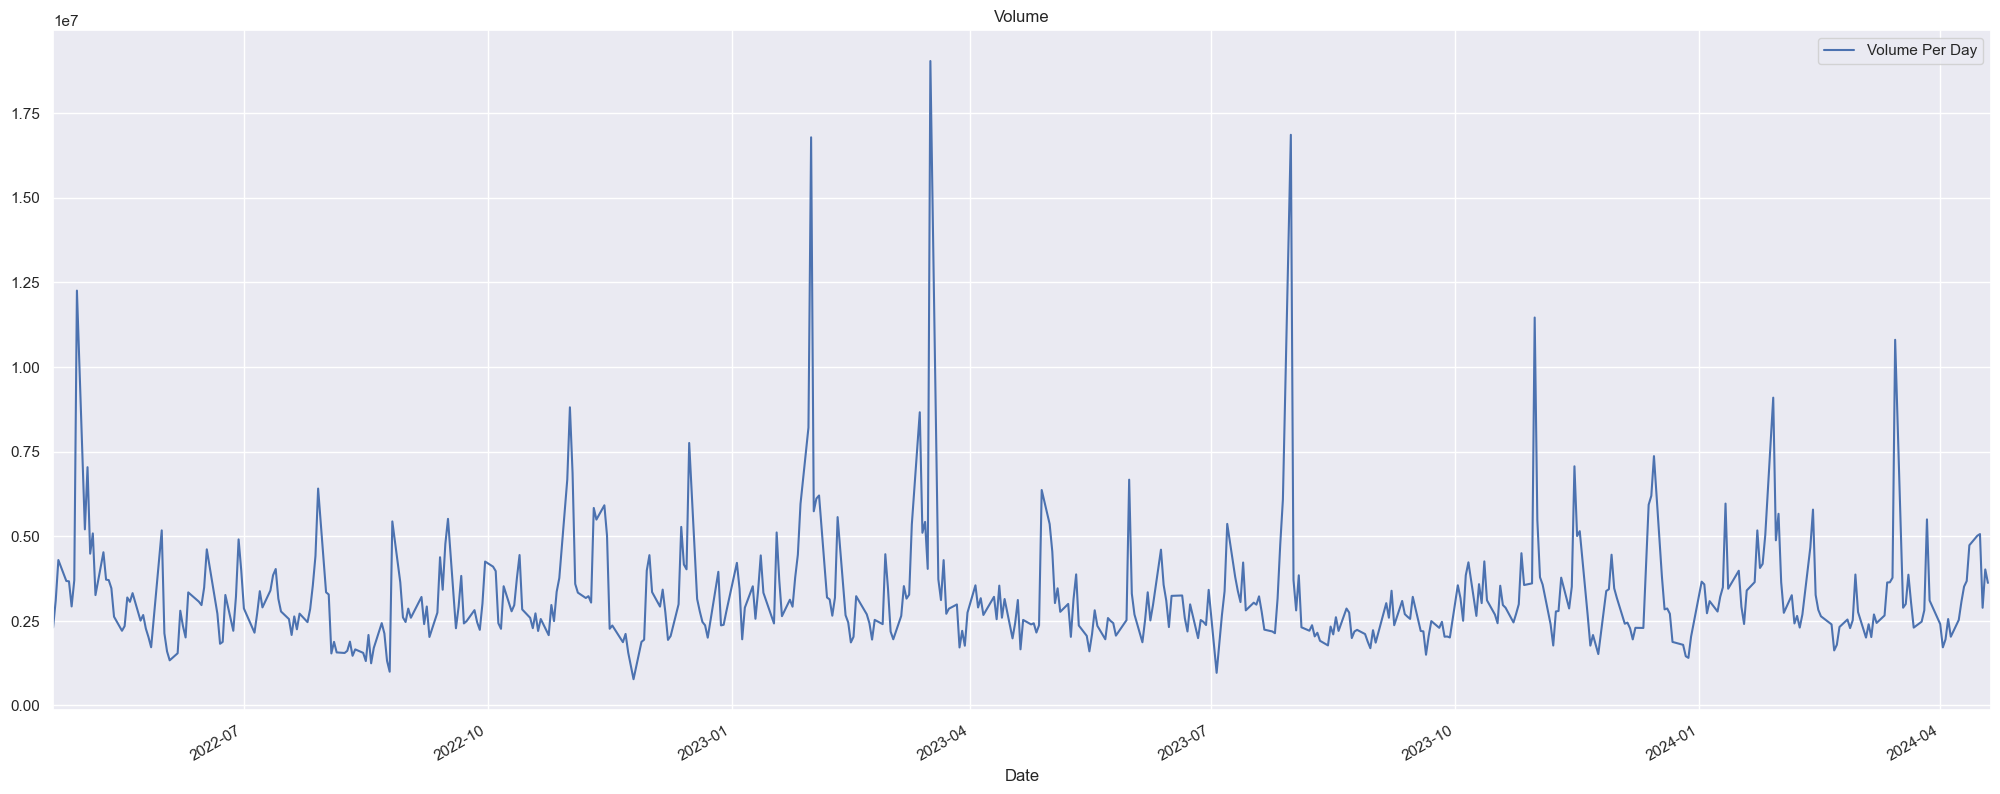
\includegraphics[width=0.85\columnwidth]{images/VolumeDataSet1d.png}
                \caption{This chart represents the Volume of stock per day from 2022-04-20 to 2024-04-20.}
                \label{fig:figure}
            \end{figure}

            \begin{figure}[H]
                \centering
                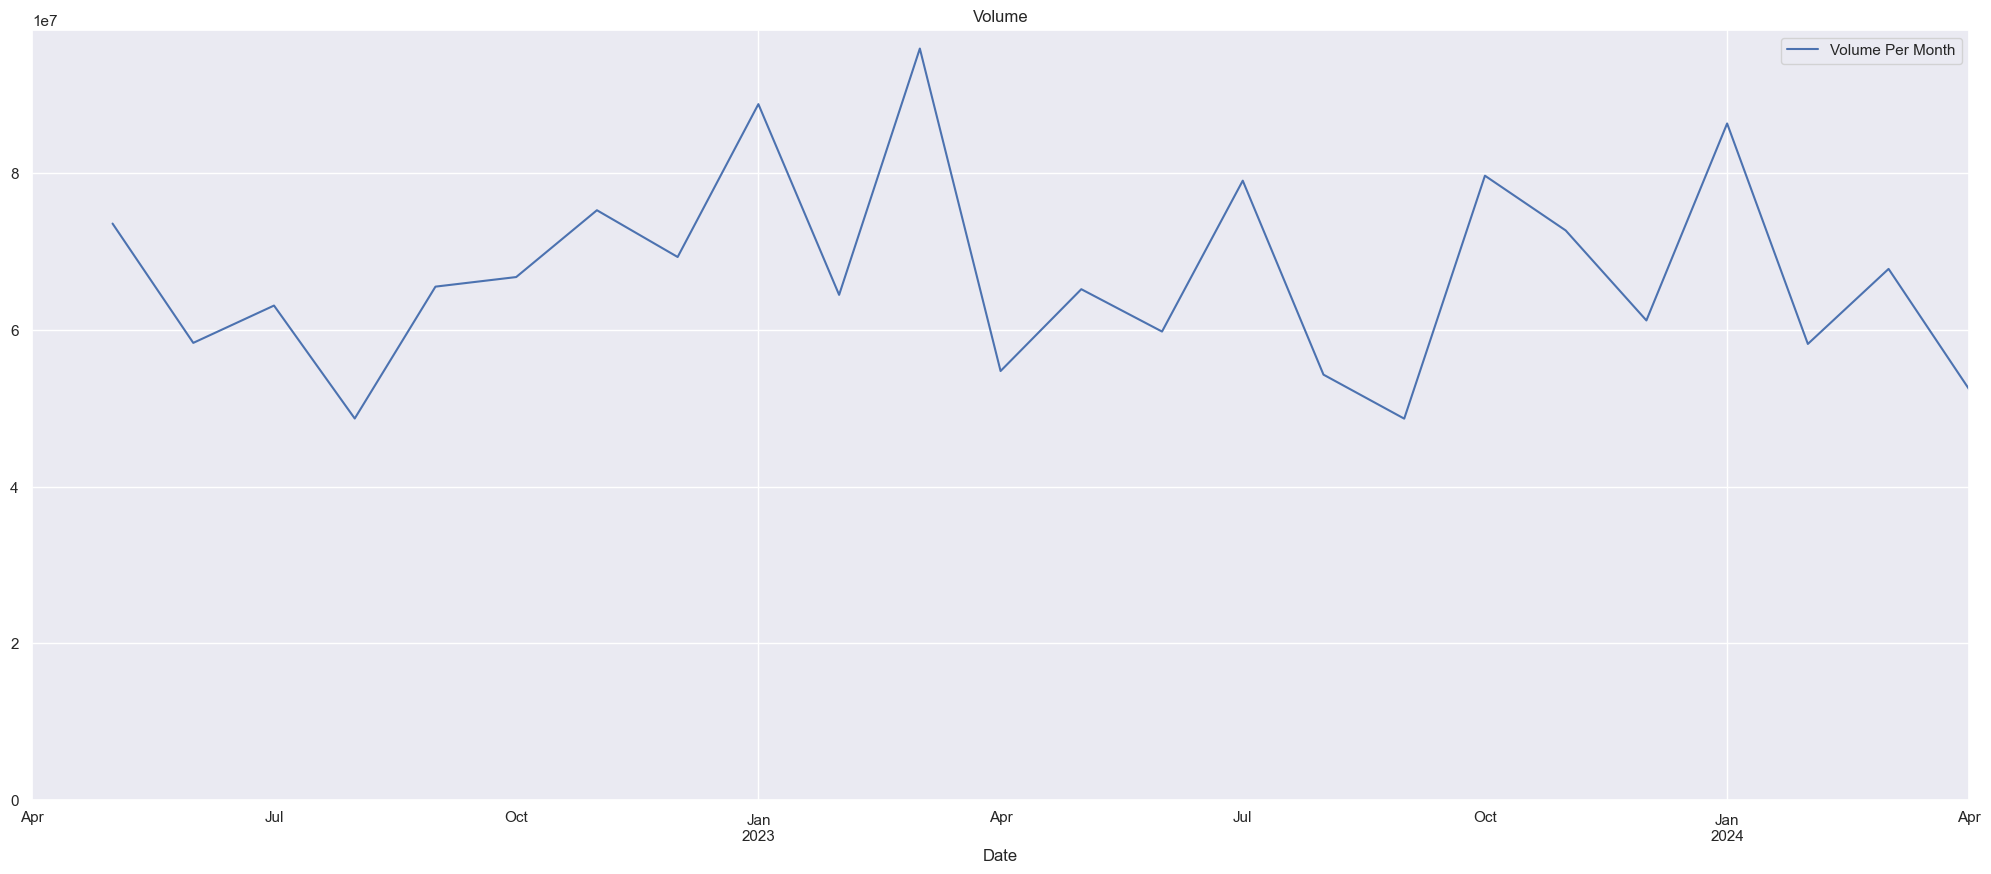
\includegraphics[width=0.85\columnwidth]{images/VolumeDataSet1mo.png}
                \caption{This chart represents the Volume of stock per month from 2022-04-20 to 2024-04-20.}
                \label{fig:figure}
            \end{figure}

            \begin{figure}[H]
                \centering
                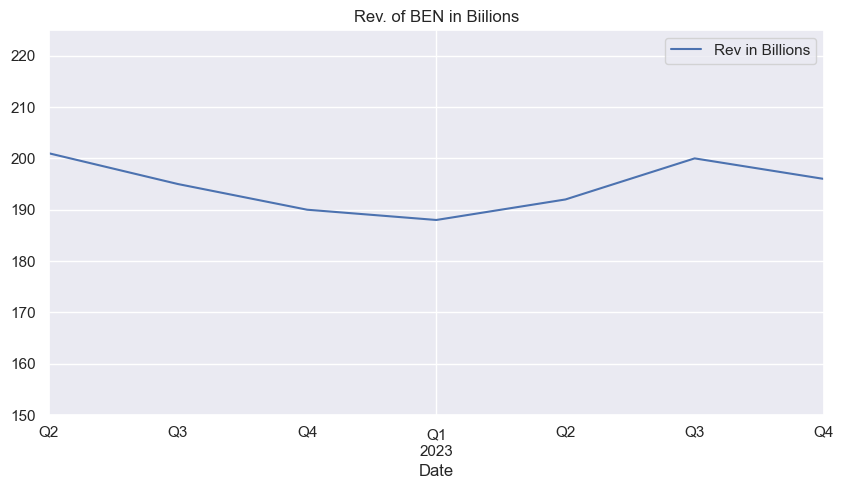
\includegraphics[width=0.85\columnwidth]{images/RevInBillions.png}
                \caption{This chart represents the Volume of stock per month vs. Volume of stock per day from 2022-04-20 to 2024-04-20.}
                \label{fig:figure}
            \end{figure}
            


            \begin{figure}[H]
                \centering
                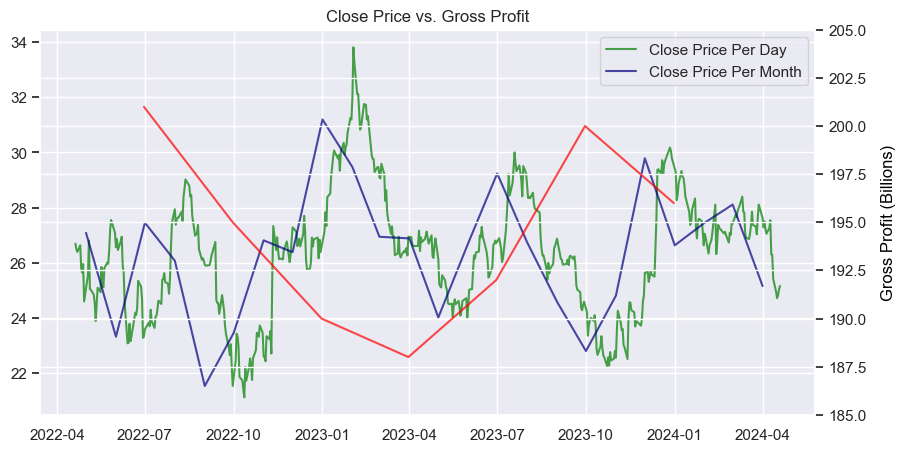
\includegraphics[width=0.85\columnwidth]{images/CloseDataVsProfit.png}
                \caption{This chart compares the monthly and daily closing price against the reported quartly earning price (in red) 2022-04-20 to 2024-04-20.}
                \label{fig:figure}
            \end{figure}



        \subsubsection{Tables}
    
            The \verb*|\captionsetup[table]| command customizes the appearance of the captions for tables in the document. The \verb*|\tabletext{}| is used to add notes to tables easily. Table \ref{tab:table}, shows an example table.
            
            \begin{table}[H]
                \centering
                \caption{Small table example.}
    		\label{tab:table}
                \begin{tabular}{cc}
            	\toprule
                    \textbf{Column 1} & \textbf{Column 2} \\
                    \midrule
                    Data 1 & Data 2 \\
                    Data 3 & Data 4 \\
                    \bottomrule
                \end{tabular}
                    
                \tabletext{Note: I'm a table text for additional information.}
                    
            \end{table}

    \subsection{Equation}
    
        Equation \ref{ec:equation} shows an example equation. 

	\begin{equation} \label{ec:equation}
            \frac{\hbar^2}{2m}\nabla^2\Psi + V(\mathbf{r})\Psi = -i\hbar \frac{\partial\Psi}{\partial t}
	\end{equation} 

        The \textbf{amssymb} package was not necessary to include, because the stix2 font incorporates mathematical symbols for writing quality equations. In case you choose another font, uncomment the package in \textit{tau class} code.

        If you want to change the values that adjust the spacing above and below in the equations, go to \textit{tau class-math packages} section and play with \verb|\setlength{\eqskip}{6.5pt}| value until the preferred spacing is set. See appendix for more information.

\section{Environment}

    The \textit{tau class} includes custom environments designed to enhance the presentation of information within documents. Among these custom environments are \textbf{tauenv}, \textbf{info} and \textbf{note}.

    \begin{tauenv}[frametitle=Custom title]
        This is an example of the custom title environment. To add a title type \verb|[frametitle=Custom title]| next to the beginning of the environment (as shown in this example).
    \end{tauenv}

    One of the main features of the info and note environment is that they automatically change the language of their titles (currently English and Spanish).

\section{Coding}

    \textit{Tau class} includes the \textit{listings} package, which offers versatile and customizable features for typesetting code snippets in \LaTeX\ documents. Specifically for C, C++, \LaTeX\ and Matlab codes. 

    For C and C++ codes, the \textit{listings} package recognizes the syntax of these programming languages and highlights keywords, comments, and string literals accordingly.

    \lstinputlisting[caption=Example of C code., language=C]{example.c}

    Similarly, for Matlab codes, the \textit{listings} package offers syntax highlighting and line numbering, to the MATLAB language syntax.
    
    \lstinputlisting[caption=Example of matlab code., language=Matlab]{example.m}

\section{References}

    The default formatting for references follows the IEEE style. This style is commonly used for technical documents, research papers, and scholarly articles in engineering fields \cite{einstein}.

    At the end of the document, you will find an example of the default reference formatting \cite{dirac}.
        
\section{Appendix}

    \subsection{Environments preview}

        The following environments are defined in \textit{tauenvs} package.
		
		\subsubsection{Tau environment}

                The following code defines the tauenv environment. A custom title can be added to this environment.

			\begin{tauenv}[frametitle=Tauenv]
                    Lorem ipsum dolor sit amet, consectetur adipiscing elit. Sed vestibulum justo quis massa aliquet, ut ultrices quam bibendum.
			\end{tauenv}
		
\begin{lstlisting}[language=TeX, caption=Tauenv environment code.]
\newmdenv[
	backgroundcolor=taublue!22, 					
	linecolor=taublue,									
	linewidth=0.7pt,
	frametitle=\vskip0pt\bfseries,
	frametitlerule=false,
	frametitlefont=\color{taublue}\bfseries\sffamily,
	frametitlealignment=\raggedright,
	innertopmargin=3pt,
	innerbottommargin=6pt,
	innerleftmargin=6pt,
	innerrightmargin=6pt,
	font=\selectfont,
	fontcolor=taublue,									
	frametitleaboveskip=8pt,
	skipabove=10pt
]{tauenv} \end{lstlisting}
		
		\subsubsection{Note}

                This code defines the note environment.

  			\begin{note}
                    Lorem ipsum dolor sit amet, consectetur adipiscing elit. Sed vestibulum justo quis massa aliquet, ut ultrices quam bibendum.
			\end{note}
		
\begin{lstlisting}[language=TeX, caption=Note environment code.]
\newmdenv[
	backgroundcolor=taublue!22, 						
	linecolor=taublue,									
	linewidth=0.7pt,
	frametitle=\vskip0pt\bfseries\notelanguage,
	frametitlerule=false,
	frametitlefont=\color{taublue}\bfseries\sffamily,
	frametitlealignment=\raggedright,
	innertopmargin=3pt,
	innerbottommargin=6pt,
	innerleftmargin=6pt,
	innerrightmargin=6pt,
	font=\normalfont,
	fontcolor=taublue,									
	frametitleaboveskip=3pt,
	skipabove=10pt
]{note} \end{lstlisting}

		\subsubsection{Info}

                This code defines the info environment.

    		\begin{info}
                    Lorem ipsum dolor sit amet, consectetur adipiscing elit. Sed vestibulum justo quis massa aliquet, ut ultrices quam bibendum.
			\end{info}
		
\begin{lstlisting}[language=TeX, caption=Info environment code.]
\newmdenv[
	backgroundcolor=taublue!22, 						
	linecolor=taublue,									
	linewidth=0.7pt,
	frametitle=\vskip0pt\bfseries\infolanguage,
	frametitlerule=false,
	frametitlefont=\color{taublue}\bfseries\sffamily,
	frametitlealignment=\raggedright,
	innertopmargin=3pt,
	innerbottommargin=6pt,
	innerleftmargin=6pt,
	innerrightmargin=6pt,
	font=\normalfont,
	fontcolor=taublue,									
	frametitleaboveskip=3pt,
	skipabove=10pt
]{info} \end{lstlisting}

    \subsection{Alternative title}

         You can make the following modification to \textit{tau class} in the \textit{title preferences} section to change the position of the title. This will move the title to the left. 

\begin{lstlisting}[language=TeX, caption=Alternative title.]
\renewcommand{\@maketitle}{%
        \vskip-18pt
    {\RaggedRight\bfseries\color{taublue}\fontsize{18}{22}\sffamily\selectfont\@title\par}
		\vskip8pt
    {\RaggedRight\normalsize\sffamily\@author\par}
        \vskip8pt
    {\RaggedRight\fontsize{7pt}{8pt}\selectfont\@professor\par}
        \vskip24pt
}% 
\end{lstlisting}

    \subsection{Equation skip value}

        Play with the value of \verb|\eqskip| until the preferred spacing is set for equations.

\begin{lstlisting}[language=TeX, caption=Equation skip code.]
\newlength{\eqskip}\setlength{\eqskip}{6.5pt}
\expandafter\def\expandafter\normalsize\expandafter{%
    \normalsize%
    \setlength\abovedisplayskip{\eqskip}%
    \setlength\belowdisplayskip{\eqskip}%
    \setlength\abovedisplayshortskip{\eqskip-\baselineskip}%
    \setlength\belowdisplayshortskip{\eqskip}%
}
\end{lstlisting}
					
%----------------------------------------------------------

\addcontentsline{toc}{section}{References}
\printbibliography

%----------------------------------------------------------

\begin{center}
	\vskip10pt
	Enjoy writing with tau \LaTeX\ class $\blacksmiley$ \\ 
	\vskip10pt
	\textit{Contact:} \\
	\faLink\ \href{https://sites.google.com/view/memo-notess/p%C3%A1gina-principal}{https://sites.google.com/memo-notess} \\
	\faEnvelope[regular]\ memo.notess1@gmail.com \\
	\faInstagram\ memo.notess\\
\end{center}

%----------------------------------------------------------

\end{document}